\documentclass[10pt,a4paper]{article}

\usepackage[a4paper,margin=15mm,headheight=14pt]{geometry}
\usepackage{array}
\usepackage{booktabs}
\usepackage{caption}
\usepackage{enumitem}
\usepackage{fancyhdr}
\usepackage{float}
\usepackage{fontspec}
\usepackage{graphicx}
\usepackage{listings}
\usepackage{longtable}
\usepackage{microtype}
\usepackage{parskip}
\usepackage{tabularx}
\usepackage{xcolor}
\usepackage{hyperref}

\definecolor{ink}{HTML}{1F2937}
\definecolor{muted}{HTML}{64748B}
\definecolor{accent}{HTML}{006B3C}
\definecolor{secondary}{HTML}{0B7A46}
\definecolor{pale}{HTML}{EAF6EF}
\definecolor{line}{HTML}{CBD5E1}
\definecolor{warm}{HTML}{FFF8E8}

\hypersetup{
  colorlinks=true,
  linkcolor=accent,
  urlcolor=secondary,
  pdftitle={TokTickIT Lab 4 Report},
  pdfauthor={GUNTEE DOUNGMANEE},
}

\setmainfont{Latin Modern Roman}
\setlength{\parindent}{0pt}
\setlist{nosep,leftmargin=*}
\setlist[itemize]{label=\textcolor{accent}{\small\textbullet}}
\newcolumntype{Y}{>{\raggedright\arraybackslash}X}
\lstdefinestyle{testoutput}{
  basicstyle=\ttfamily\scriptsize,
  breaklines=true,
  breakatwhitespace=true,
  columns=fullflexible,
  keepspaces=true,
  showstringspaces=false,
  frame=single,
  framesep=3pt,
  aboveskip=4pt,
  belowskip=4pt
}
\lstdefinestyle{testoutputsmall}{
  style=testoutput,
  basicstyle=\ttfamily\tiny
}

\pagestyle{fancy}
\fancyhf{}
\lhead{TokTickIT Lab 4}
\rhead{Actions Taken, dashboards, regression}
\cfoot{\thepage}
\renewcommand{\headrulewidth}{0.3pt}

\newcommand{\answerpart}[2]{%
  \clearpage
  \section*{Answer Part #1: #2}%
  \addcontentsline{toc}{section}{Answer Part #1: #2}%
}
\newcommand{\statusnote}[1]{%
  \fcolorbox{accent}{pale}{\parbox{0.96\linewidth}{\small #1}}%
}
\newcommand{\screenshotlink}[2]{%
  \href{https://github.com/ovenmakemeheat/toktickit/blob/bd8cecd63f1dd3386b0b7f2ffcf270805e0190f3/#1}{#2}%
}
\newcommand{\reportlink}[2]{%
  \href{https://github.com/ovenmakemeheat/toktickit/blob/docs/lab4-docs/#1}{#2}%
}
\newcommand{\evidenceimage}[3]{%
  \begin{figure}[H]\centering
    \includegraphics[width=#2\linewidth,height=0.72\textheight,keepaspectratio]{#1}
    \caption{#3}
  \end{figure}%
}
\newcommand{\compactimage}[3]{%
  \begin{minipage}[t]{0.48\linewidth}\centering
    \includegraphics[width=\linewidth,height=0.35\textheight,keepaspectratio]{#1}
    \captionof{figure}{#2}\label{#3}
  \end{minipage}%
}
\newcommand{\responsivescreens}[4]{%
  \clearpage
  \subsection*{#1 -- desktop, tablet, and mobile}
  \begin{figure}[H]\centering
    \includegraphics[width=0.98\linewidth,height=0.40\textheight,keepaspectratio]{#2}
    \caption{Desktop viewport, 1440 $\times$ 900.}
  \end{figure}
  \vspace{-2mm}
  \noindent
  \begin{minipage}[t]{0.48\linewidth}\centering
    \includegraphics[width=\linewidth,height=0.32\textheight,keepaspectratio]{#3}
    \captionof{figure}{Tablet viewport, 768 $\times$ 1024}
  \end{minipage}\hfill
  \begin{minipage}[t]{0.48\linewidth}\centering
    \includegraphics[width=\linewidth,height=0.32\textheight,keepaspectratio]{#4}
    \captionof{figure}{Mobile viewport, 390 $\times$ 844}
  \end{minipage}
  \clearpage
}
\newcommand{\responsiveforms}[4]{%
  \clearpage
  \subsection*{#1 -- desktop form capture}
  \begin{figure}[H]\centering
    \includegraphics[width=0.96\linewidth,height=0.72\textheight,keepaspectratio]{#2}
    \caption{Action Taken panel at 1440 $\times$ 900.}
  \end{figure}
  \clearpage
  \subsection*{#1 -- tablet and mobile form captures}
  \begin{minipage}[t]{0.48\linewidth}\centering
    \includegraphics[width=\linewidth,height=0.67\textheight,keepaspectratio]{#3}
    \captionof{figure}{Action Taken panel at 768 $\times$ 1024}
  \end{minipage}\hfill
  \begin{minipage}[t]{0.48\linewidth}\centering
    \includegraphics[width=\linewidth,height=0.67\textheight,keepaspectratio]{#4}
    \captionof{figure}{Action Taken panel at 390 $\times$ 844}
  \end{minipage}
  \clearpage
}
\newcommand{\evidencepath}[1]{\texttt{\path{#1}}}

\begin{document}

\begin{titlepage}
  \thispagestyle{empty}
  \vspace*{16mm}
  {\Large\textcolor{accent}{CPE 334 \textbar\ Lab 4}\par}
  \vspace{8mm}
  {\Huge\bfseries TokTickIT\par}
  \vspace{3mm}
  {\Large Actions Taken, dashboards, and final regression\par}
  \vspace{5mm}
  {\large Release evidence and demonstration report\par}
  \vfill
  \begin{tabular}{@{}>{\bfseries}p{40mm}p{110mm}@{}}
    Student & GUNTEE DOUNGMANEE \\
    Student ID & 67070501003 \\
    Peer reviewer & MadMax168 (GitHub) \\
    Repository & \href{https://github.com/ovenmakemeheat/toktickit}{ovenmakemeheat/toktickit} \\
    Parent issue & \href{https://github.com/ovenmakemeheat/toktickit/issues/86}{\#86 -- Lab 4} \\
    Report branch & \path{docs/lab4-docs} \\
    Release source & \path{main}, \texttt{bd8cecd} (PR \#98) \\
    Stack & React, TypeScript, Vite, Express, Prisma, PostgreSQL \\
  \end{tabular}
  \vfill
  \statusnote{\textbf{Release source:} PR \#98 merged \path{lab4-staging} into \path{main} on 2026-10-29 at \texttt{bd8cecd63f1dd3386b0b7f2ffcf270805e0190f3}. The report is prepared on \path{docs/lab4-docs} from the release source tree.}
  \vfill
  {\small This PDF uses the required Answer Part 1 through Answer Part 9 headings in order.}
\end{titlepage}

\tableofcontents
\clearpage

\answerpart{1}{Git Use with Engineering Workflow}

Lab 4 used one feature branch per approved issue, integrating feature Pull Requests into \path{lab4-staging} before the release Pull Request to \path{main}. The table lists linked branches, associated Pull Requests, and merge destinations.

\begin{center}\small
\begin{tabularx}{\linewidth}{@{}p{34mm}p{66mm}Y@{}}
\toprule
Issue & Feature branch / PR & Integration \\
\midrule
\href{https://github.com/ovenmakemeheat/toktickit/issues/87}{\#87 Contract} & \path{feature/20-lab4-contract-}\newline\path{test-plan}; \href{https://github.com/ovenmakemeheat/toktickit/pull/91}{PR \#91} & Merged to \path{lab4-staging} at \href{https://github.com/ovenmakemeheat/toktickit/commit/c945062c41b2fa85b8f279cc7cc852e07a5aa8fb}{\texttt{c945062}} before implementation PRs. \\
\href{https://github.com/ovenmakemeheat/toktickit/issues/88}{\#88 Actions/workflow} & \path{feature/21-lab4-actions-}\newline\path{taken-ticket-workflow}; \href{https://github.com/ovenmakemeheat/toktickit/pull/92}{PR \#92} & Merged to \path{lab4-staging} at \href{https://github.com/ovenmakemeheat/toktickit/commit/8608a312d298ecfd480ea67b0fe9ffd5ccf5db5f}{\texttt{8608a31}}. \\
\href{https://github.com/ovenmakemeheat/toktickit/issues/89}{\#89 Dashboards} & \path{feature/22-lab4-role-}\newline\path{dashboards}; \href{https://github.com/ovenmakemeheat/toktickit/pull/93}{PR \#93} & Merged to \path{lab4-staging} at \href{https://github.com/ovenmakemeheat/toktickit/commit/47d6487b638939835403ea0da7c0e3f011078b7b}{\texttt{47d6487}}. \\
\href{https://github.com/ovenmakemeheat/toktickit/issues/90}{\#90 Regression/readiness} & \path{feature/23-lab4-regression-}\newline\path{demo-readiness}; \href{https://github.com/ovenmakemeheat/toktickit/pull/94}{PR \#94} & PR \#94 merged to staging at \href{https://github.com/ovenmakemeheat/toktickit/commit/7cb171562bac42e7dce9cf7d5aee42022de9e253}{\texttt{7cb1715}}; follow-ups \href{https://github.com/ovenmakemeheat/toktickit/pull/95}{\#95}, \href{https://github.com/ovenmakemeheat/toktickit/pull/96}{\#96}, \href{https://github.com/ovenmakemeheat/toktickit/pull/97}{\#97} also merged to staging. \\
Release & \path{lab4-staging}; \href{https://github.com/ovenmakemeheat/toktickit/pull/98}{PR \#98} & Merged by MadMax168 into \path{main} on 2026-10-29 at \href{https://github.com/ovenmakemeheat/toktickit/commit/bd8cecd63f1dd3386b0b7f2ffcf270805e0190f3}{\texttt{bd8cecd}}. \\
\bottomrule
\end{tabularx}
\end{center}

The release commit is \href{https://github.com/ovenmakemeheat/toktickit/commit/bd8cecd63f1dd3386b0b7f2ffcf270805e0190f3}{\texttt{bd8cecd}}. At release, \path{main} and \path{lab4-staging} had identical Git trees. As captured on 2026-10-29, all Lab 4 issues \#86--\#90 are closed; parent issue \#86 is in \texttt{Done} on the public \href{https://github.com/users/ovenmakemeheat/projects/4/views/1}{Lab 4 Project Kanban}, with native sub-issue progress at 4/4 (100\%). The board screenshot below records the visible final state. Native sub-issues remain attached to the parent and are not separate board items.

\begin{figure}[H]\centering
  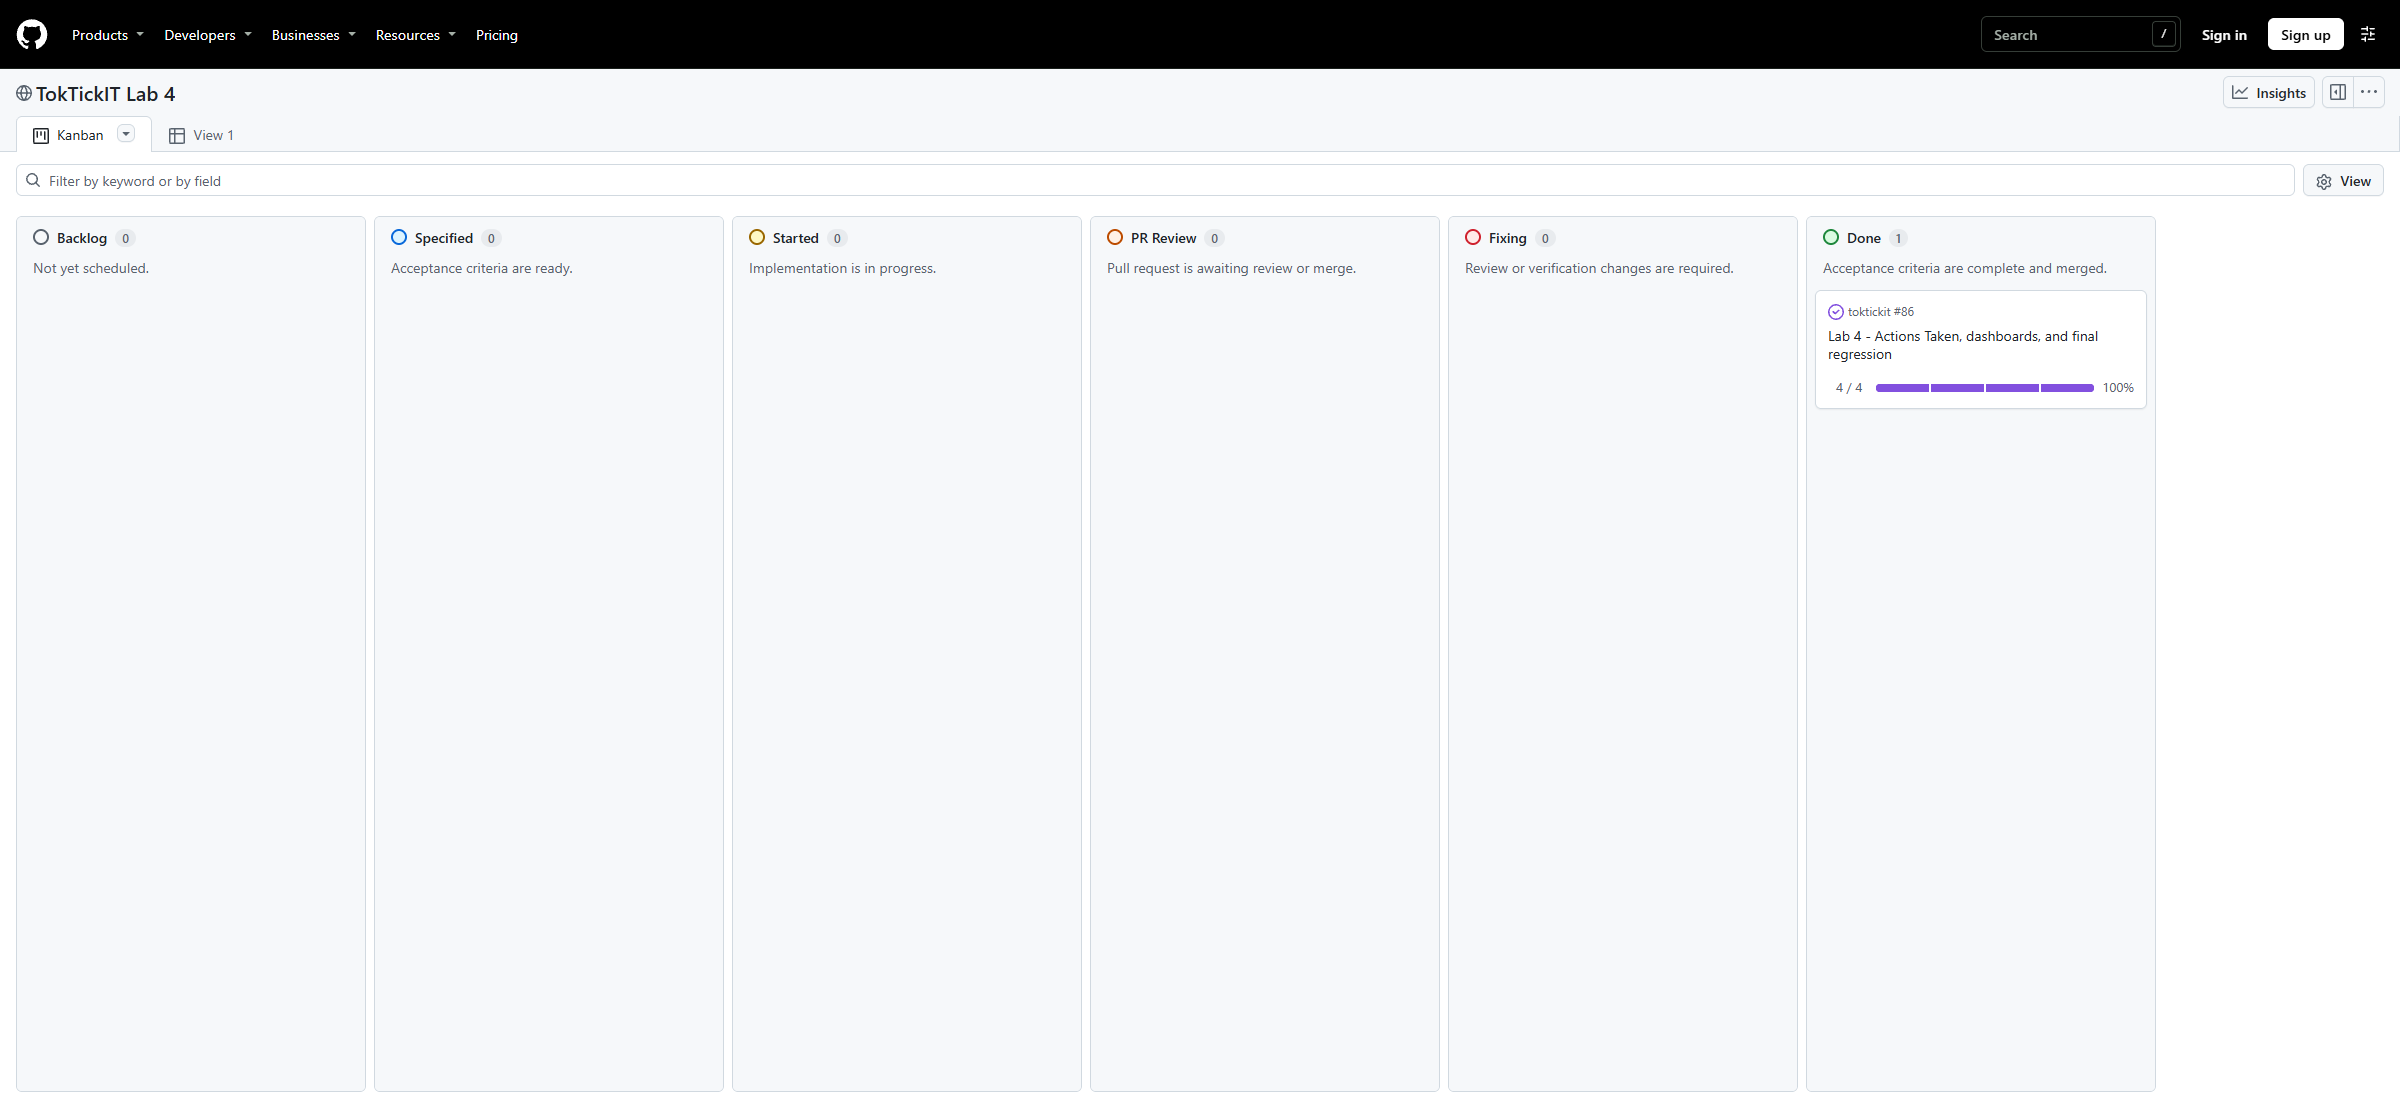
\includegraphics[width=0.98\linewidth,height=0.34\textheight,keepaspectratio]{docs/lab-04/report/evidence/lab4-project-kanban.png}
  \caption{Lab 4 Project Kanban captured 2026-10-29: parent issue \#86 is in Done and reports 4/4 sub-issues complete.}
\end{figure}

\subsection*{Reviewer and repository evidence}

The feature and release Pull Requests are linked in the table above; MadMax168 is identified as peer reviewer, and PR \#98 records the release merge to \path{main}. The engineering contract PR \#91 predates implementation PRs \#92--\#94. The report branch is based on the released source tree and contains this documentation work.

\begin{quote}\small
\textbf{Repository structure at release:} \path{client/} (React application and UI tests); \path{server/} (Express API, Prisma schema/migrations, and API tests); \path{e2e/} (Playwright journeys); \path{docs/lab-04/} (engineering contract, test plan, evidence, and report); \path{artifacts/lab-04/} (visual and machine-readable release evidence).
\end{quote}

The linked \href{https://github.com/ovenmakemeheat/toktickit/blob/bd8cecd63f1dd3386b0b7f2ffcf270805e0190f3/README.md}{README} documents Bun/Docker setup, migration, seed, test database, local demonstration, and verification commands. The linked \href{https://github.com/ovenmakemeheat/toktickit/blob/bd8cecd63f1dd3386b0b7f2ffcf270805e0190f3/.gitignore}{\texttt{.gitignore}} excludes environment secrets, local database/storage state, build and test output, and LaTeX intermediates.

\answerpart{2}{Spec DD}

The Lab 4 engineering contract converts the handout into a bounded, testable increment. The contract existed and was integrated through PR \#91 before the dependent implementation PRs. It covers \textbf{FR-01--FR-20}, \textbf{BR-01--BR-25}, and \textbf{AC-01--AC-26}; the complete rendered source is \reportlink{docs/lab-04/specification.md}{\texttt{specification.md}}, with supporting \reportlink{docs/lab-04/api-spec.md}{API}, \reportlink{docs/lab-04/ui-spec.md}{UI}, and \reportlink{docs/lab-04/tests.md}{test} contracts.

\begin{itemize}
  \item \textbf{Actions Taken:} child of exactly one Ticket; actor derived from the authenticated session; action time and stable chronological order; required description/result; conditional follow-up note; optional plain-text Attachment Notes; idempotent creation; versioned edits; no deletion.
  \item \textbf{Workflow:} only IT Staff/Admin may transition status; required confirmations are explicit; `RESOLVED` requires real work, and re-resolution after reopening requires a newly created Action Taken. Requester resolution indication remains advisory.
  \item \textbf{Dashboards:} requester-owned metrics and staff/admin operational metrics are computed server-side using one `asOf` and an inclusive rolling 30-day UTC window. Recent lists are bounded to five rows and drill into existing detailed screens.
  \item \textbf{Preservation:} additive migration retains Lab 3 rows and relationships, fabricates no work history, and documents timestamp approximations for legacy resolved/closed/reopened Tickets. Seed behavior is repeat-safe.
\end{itemize}

Two consequential database choices are an immutable `createdAt` boundary for the post-reopen work gate (because editable `actionAt` does not establish when a record was added) and a separate `resolvedAt` value (because comments/actions can update Ticket activity without changing resolution time). The migration adds `lastReopenedAt` as an internal marker and avoids a destructive rollback after new work records exist.

\subsection*{Numbered requirements and acceptance coverage}
\begin{center}\scriptsize
\begin{tabularx}{\linewidth}{@{}p{17mm}Y@{}}
\toprule
ID & Contracted behavior \\
\midrule
FR-01 & IT Staff/Admin create Actions Taken; performer comes from the authenticated session. \\
FR-02 & Store action time, description, result, follow-up flag/note, and Attachment Notes. \\
FR-03 & Requesters read work only on owned Tickets; no Action Taken writes. \\
FR-04 & Staff/Admin edits preserve original performer, Ticket, and creation data. \\
FR-05 & Stable ordering, idempotent create, and stale-edit conflicts. \\
FR-06 & No Action Taken delete operation. \\
FR-07 & Server-enforced status matrix and confirmations. \\
FR-08 & Resolution requires real work; Requester signal is advisory. \\
FR-09 & Track resolution and reopen timestamps with documented legacy backfill. \\
FR-10 & Requester dashboard contains only authenticated Requester metrics/summaries. \\
FR-11 & Staff/Admin dashboard uses owner, status, priority, and current-user filters. \\
FR-12 & Dashboards return bounded summaries and actionable drill-downs. \\
FR-13 & Dashboard calculations use a single server-side UTC window. \\
FR-14 & Additive migration preserves Lab 3 data; no fabricated Actions Taken. \\
FR-15 & Repeat-safe seed covers representative statuses and zero/non-zero data. \\
FR-16 & Lab 1--3 authentication, role, Ticket, attachment, comment, note, and admin behavior remains. \\
FR-17 & Role screens remain keyboard/assistive-technology usable and responsive. \\
FR-18 & Acceptance evidence maps to tests, commands, and manual checks. \\
FR-19 & Staff/Admin `myRecentActions` is performer-scoped, status-independent, and bounded. \\
FR-20 & Release hardening checks role navigation, page errors, links, and unfinished UI. \\
\bottomrule
\end{tabularx}
\end{center}

\begin{center}\small
\begin{tabularx}{\linewidth}{@{}p{25mm}Y@{}}
\toprule
Rule / criteria & Summary and test trace \\
\midrule
BR-01--BR-15 & Ticket-owned Action Taken data, immutable actor/parent/fingerprint, editable audit fields, follow-up rules, stable order, idempotency, versions, role/ownership enforcement, and atomic activity updates. Verified by UNIT-01, API-01--04, E2E-01. \\
BR-16--BR-24 & Complete transition matrix; confirmation; Action Taken resolution gate; `resolvedAt`/`lastReopenedAt`; atomic status conflict; legacy Tickets stay valid. Verified by UNIT-02, API-05/API-08, E2E-02. \\
BR-25; AC-25 & Current-user `My Recent Actions` is performer-scoped rather than owner-scoped, includes every Ticket status, observes inclusive 30-day UTC bounds, sorts newest-first, and caps at five. Verified by API-07, UI-02, E2E-03, PERF-01. \\
AC-01--AC-09 & Action Taken create/read/update, role boundaries, safe attachment notes, idempotency, and stale-version behavior. Verified by UNIT-01, API-01--04, UI-01, E2E-01. \\
AC-10--AC-12 & Status matrix, resolution/reopen gates, confirmation, and concurrent status conflict. Verified by UNIT-02, API-05, E2E-02. \\
AC-13--AC-17 & Requester and operational dashboard query scopes, calculations, bounded rows, destinations, and Admin capability retention. Verified by API-04/API-06/API-07, UI-02/UI-03, E2E-03/E2E-04. \\
AC-18--AC-24 & UI states, Labs 1--3 regression, migration/seed, responsive/accessibility, performance, and contract evidence. Verified by UI-01--03, API-08, PERF-01, VIS-01, DOC-01. \\
AC-26 & Representative seeded release routes have role/API evidence, zero unexpected page/console errors, working navigation, and no visible placeholder text. Verified by E2E-04 and VIS-01. \\
\bottomrule
\end{tabularx}
\end{center}

\textbf{Product Definition of Done:} the implemented features, migration/recovery tests, seeded regression suite, responsive/accessibility inspection, prior-Lab regression, and setup/demo documentation are recorded complete. At report capture, issues \#86--\#90 were closed and the Kanban placed parent \#86 in Done with all four native sub-issues complete; see the board evidence above.

\answerpart{3}{Test DD and Traceability}

The acceptance criteria map to named unit, API/integration, UI, E2E, performance, visual, and documentation checks in \reportlink{docs/lab-04/tests.md}{\texttt{tests.md}}. Representative files include:

\begin{center}\small
\begin{tabularx}{\linewidth}{@{}p{27mm}Y@{}}
\toprule
Coverage & Actual test files \\
\midrule
Actions Taken validation, persistence, actor/owner, idempotency, edit conflicts & \evidencepath{server/tests/lab-04/actions-taken.unit.test.ts}; \evidencepath{server/tests/lab-04/actions-taken.api.test.ts}; \evidencepath{client/tests/lab-04/ActionsTaken.test.tsx} \\
Ticket transition/resolution rules and role access & \evidencepath{server/tests/lab-04/ticket-workflow.api.test.ts}; \evidencepath{client/tests/lab-04/TicketWorkflow.test.tsx} \\
Requester and operational dashboard metrics & \evidencepath{server/tests/lab-04/requester-dashboard.api.test.ts}; \evidencepath{server/tests/lab-04/staff-dashboard.api.test.ts}; \evidencepath{client/tests/lab-04/RequesterDashboard.test.tsx}; \evidencepath{client/tests/lab-04/StaffDashboard.test.tsx} \\
Migration, seed recovery, and performance smoke & \evidencepath{server/tests/lab-04/migration-seed.api.test.ts}; \evidencepath{server/tests/lab-04/dashboard-performance.api.test.ts} \\
Real seeded E2E and prior-Lab regression & \evidencepath{e2e/lab-04/actions-taken-flow.spec.ts}; \evidencepath{e2e/lab-04/ticket-resolution.spec.ts}; \evidencepath{e2e/lab-04/dashboards.spec.ts}; \evidencepath{e2e/lab-04/prior-labs-regression.spec.ts}; Lab 2/3 release suites \\
\bottomrule
\end{tabularx}
\end{center}

\textbf{Executed against release source} \texttt{bd8cecd63f1dd3386b0b7f2ffcf270805e0190f3}, from the report branch with the same product tree as \path{main}. `bun run verify` passed: Biome checked 142 files; Lefthook and Prisma validation passed; client/server type checks and builds passed; client tests passed (19 files/72 tests); server tests passed (29 files/171 tests). `bun run test:e2e` passed all 19 Chromium tests across Labs 2--4 against isolated PostgreSQL \path{toktickit_test} on port 15434. Seeded Lab 4 journeys used real APIs without business-route mocks. E2E-04 records the release revision, zero browser/page errors, and `businessApiMocks: false`.

\textbf{Complete captured command output:} the logs below are sanitized terminal output from the passing commands. ANSI color/control sequences and non-ASCII terminal decoration are normalized for PDF rendering; test names, summaries, and command results are retained.

\subsection*{\texttt{bun run verify}}
\lstinputlisting[style=testoutput]{docs/lab-04/report/evidence/main-verify-output.txt}

\clearpage
\subsection*{\texttt{bun run test:e2e}}
\lstinputlisting[style=testoutputsmall]{docs/lab-04/report/evidence/main-e2e-output.txt}

\answerpart{4}{AI Use with Reflection}

The specification and Issue \#90 implementation sessions used OpenAI Codex.
\begin{quote}\small
Model: \texttt{gpt-6-luna} \\ Provider: \texttt{openai-codex}
\end{quote}
The full \reportlink{docs/lab-04/ai-use.md}{AI-use record} includes the human-responsibility statement. Nine selected prompts are:

\begin{enumerate}
  \item “on @docs/lab-04/requirements/UTF-8\_SE+Lab+4.pdf”
  \item “this should break down into tickets issues (use my issues format)”
  \item “make sure you keep every requirement”
  \item “create a project board for lab 4”
  \item “using kanban as main”
  \item “next let's create lab 4 staging branch”
  \item “edit issue propose branch number to increment continuing with lab3 number branch name”
  \item “now get into first branch and start implement”
  \item “Implement Issue \#90.”
\end{enumerate}

\textbf{My Reflection.} I used the specification agent to turn the Lab 4 handout into numbered requirements, business rules, acceptance criteria, and a test plan before implementation. The coding agent helped implement the approved work and prepare seeded regression journeys and release evidence. I reviewed the scope against the handout, inspected the changes, and used the verification and end-to-end results to assess the released product. A key technical lesson from the work was that `updatedAt` cannot prove new work was recorded after a Ticket is reopened: ordinary edits also change activity timestamps. The separate `lastReopenedAt` marker and Action Taken creation time make that gate testable. AI accelerated contract drafting and repetitive implementation, while I remained accountable for scope, evidence, and the final decisions.

\answerpart{5}{Working IT Staff Dashboard UI}

IT Staff and Administrators share the operational Dashboard. It reports active unassigned work, the signed-in User's owned active work, active high priority work, status and IT Priority breakdowns, recently updated Tickets, and the current User's recent Actions Taken. Calculations are server-backed, bounded, and linked to Queue/Ticket Detail destinations; the Administrator reuses the IT Staff view.

The seeded dashboard inspection recorded 18 active Tickets: 14 New, 1 Open, 1 In Progress, 1 Waiting for Requester, and 1 Reopened. IT Priority totals were 1 Low, 1 Medium, and 16 High. The same sample included 14 unassigned active Tickets, 0 assigned to the inspected IT Staff account, and 16 high-priority active Tickets. API tests compare exact query results, UTC-window boundaries, scopes, caps, and safe DTOs against deterministic database fixtures. The local populated-seed performance smoke recorded Staff 20.5 ms / 3,167 B and Requester 14.1 ms / 2,272 B; these are local measurements, not production SLOs. Loading, empty, forbidden, retryable failure, and drill-down states are covered by the client/API tests and seeded E2E suite.

\begin{minipage}[t]{0.48\linewidth}\centering
  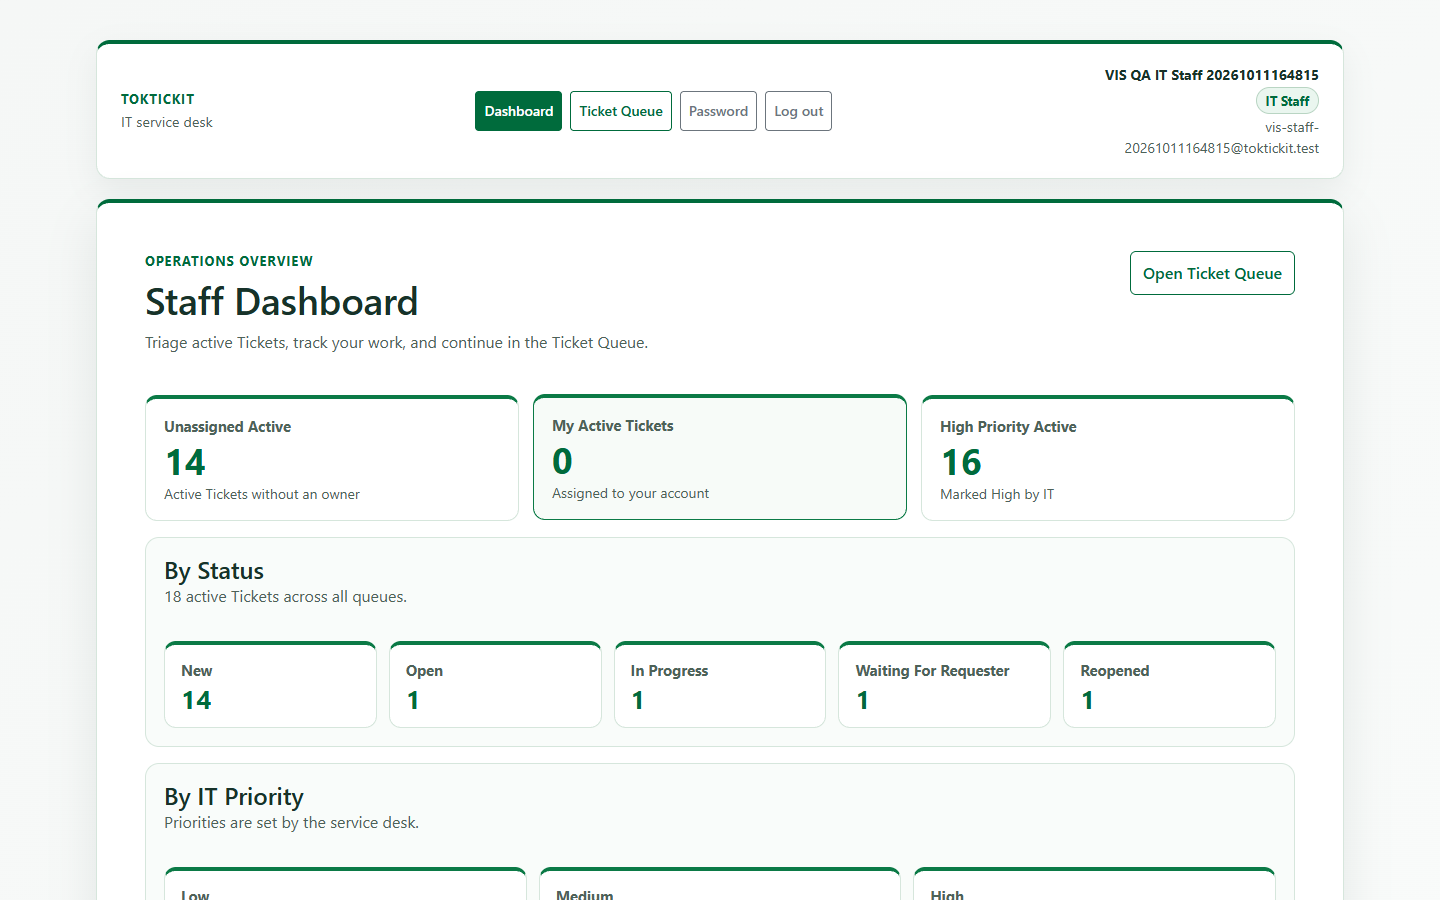
\includegraphics[width=\linewidth,height=0.31\textheight,keepaspectratio]{docs/lab-04/report/evidence/viewport/staff-dashboard-desktop.png}
  \captionof{figure}{Seeded Staff Dashboard metrics and breakdowns.}
\end{minipage}\hfill
\begin{minipage}[t]{0.48\linewidth}\centering
  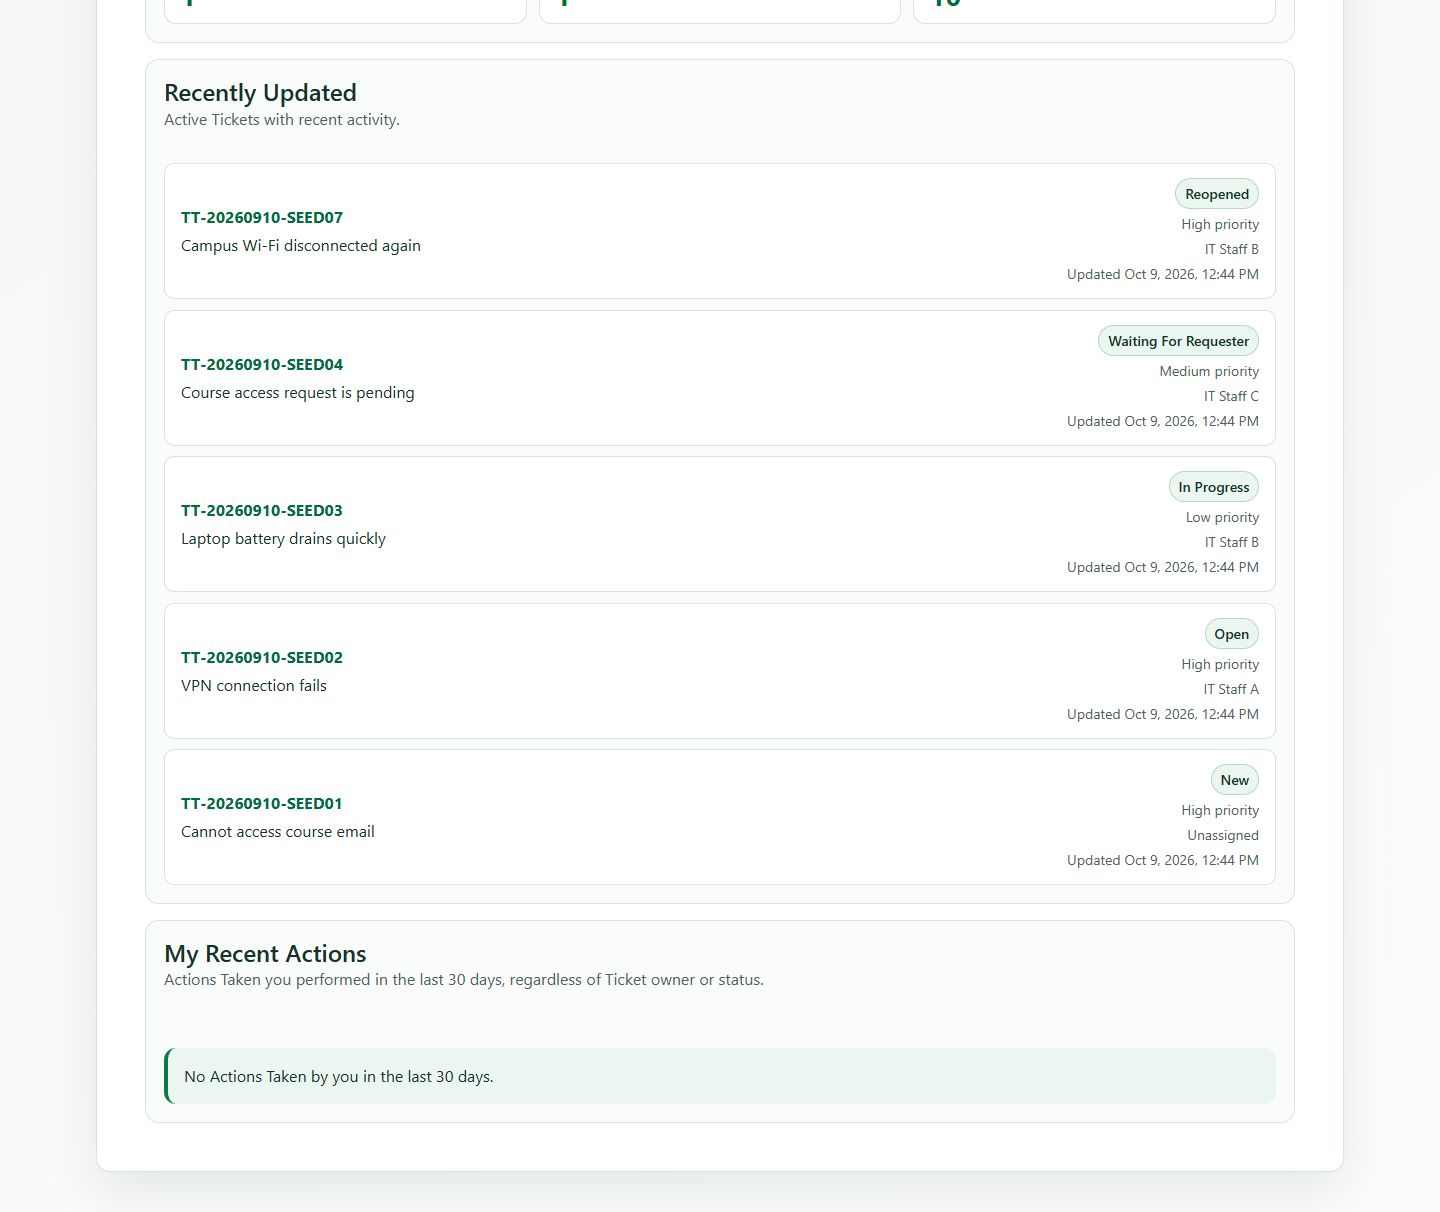
\includegraphics[width=\linewidth,height=0.31\textheight,keepaspectratio]{docs/lab-04/report/evidence/viewport/staff-dashboard-recent-lists.png}
  \captionof{figure}{Recently updated Tickets and the empty current-user Actions Taken state.}
\end{minipage}

\begin{figure}[H]\centering
  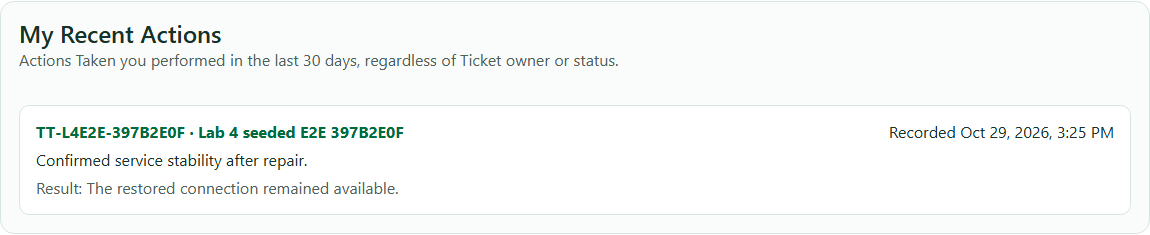
\includegraphics[width=0.92\linewidth,height=0.16\textheight,keepaspectratio]{docs/lab-04/report/evidence/staff-recent-actions-desktop.png}
  \caption{A seeded Action Taken performed by IT Staff A appears in My Recent Actions even though IT Staff B owns the resolved Ticket. Tablet and mobile component captures are also recorded.}
\end{figure}

\answerpart{6}{Working Actions Taken UI}

The staff Ticket Detail presents work history separately from public communication, private Internal Notes, and Attachments. Each Action Taken shows the authenticated performer, action time, description, result, and follow-up state. Staff/Admin may add or edit records; Requesters see owned-ticket history read-only. The API keeps the primary Ticket Owner unchanged, rejects inactive assignment targets, prevents retry duplicates, and preserves the winning edit on stale-version conflicts. There is no delete or upload control in the Action Taken section.

The seeded E2E journey creates and edits Actions Taken under real PostgreSQL, verifies Requester read-only visibility and write denial, and checks that repeated creation does not duplicate work. The visual evidence below shows two chronological work records on the same Ticket. Client/API tests cover validation, safe failures, role restrictions, follow-up note rules, plain-text Attachment Notes, and optimistic edits. Ticket Owner assignment, status changes, resolve/cancel paths, and inactive-assignee rejection are exercised by the Ticket workflow and release-regression suites; the Action Taken performer remains distinct from the Ticket Owner.

\vspace{2mm}
\begin{figure}[H]\centering
  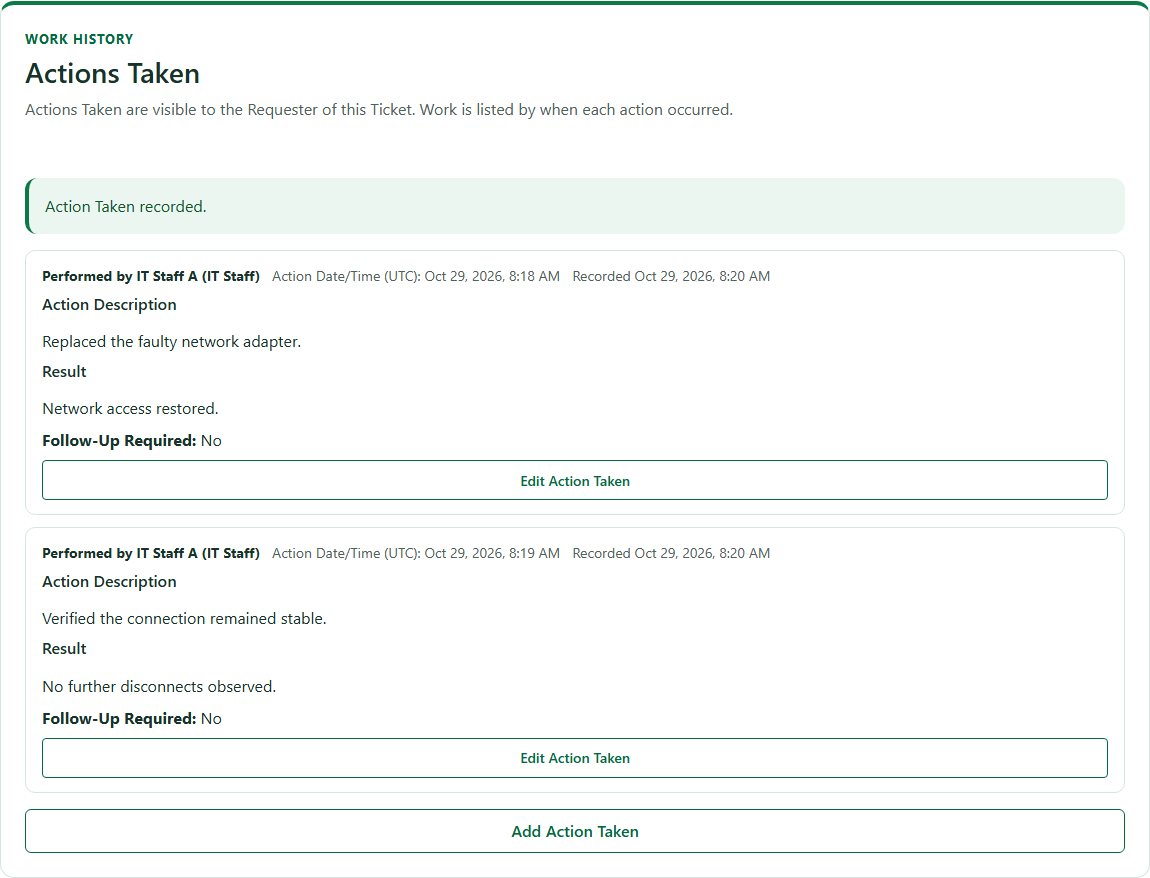
\includegraphics[width=0.76\linewidth,height=0.34\textheight,keepaspectratio]{docs/lab-04/report/evidence/actions-taken-multiple-staff.png}
  \caption{Two Actions Taken on one seeded Ticket in the Staff view. The Staff can edit each entry; creation time and action time remain distinct.}
\end{figure}
\vspace{-3mm}
\begin{figure}[H]\centering
  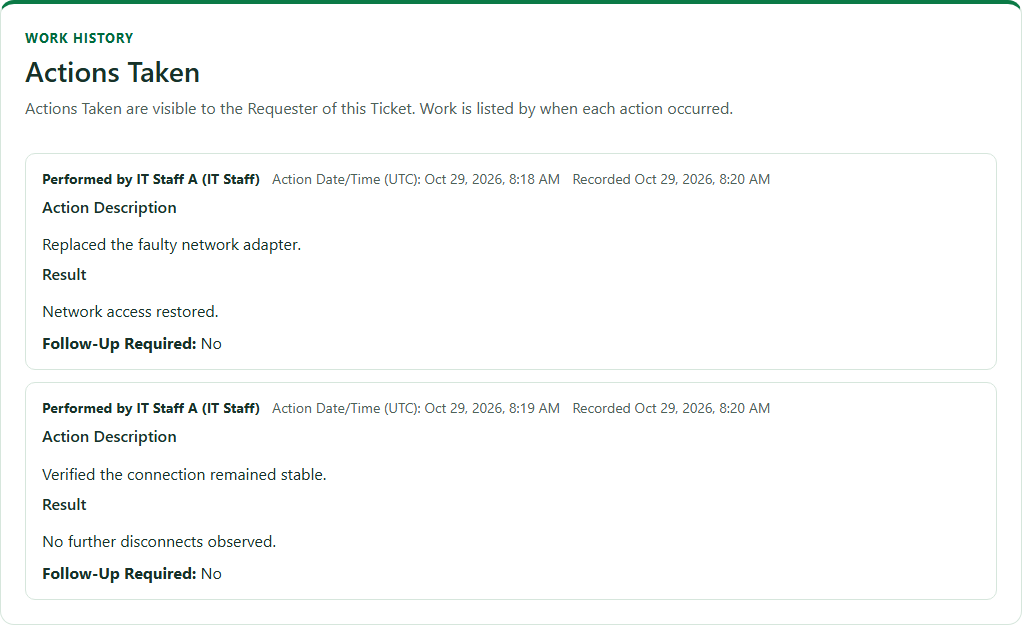
\includegraphics[width=0.76\linewidth,height=0.30\textheight,keepaspectratio]{docs/lab-04/report/evidence/actions-taken-multiple-requester.png}
  \caption{The same two Actions Taken are visible to the owning Requester; create and edit controls are absent. The test used the real API and isolated PostgreSQL. Create/edit forms at all viewports are included in Part 9.}
\end{figure}

\answerpart{7}{Working Ticket Workflow}

Only IT Staff and Administrators may perform formal transitions. The backend rejects unlisted transitions and requires explicit confirmation for resolution, closure, reopening, and cancellation. New resolution requires an Action Taken; after reopening, the work record must have been created after the latest reopen. Requester indication remains advisory. Action history orders by `actionAt`, then ID; entries are not deletable, and edits preserve original performer/creation metadata while incrementing a version.

\begin{center}\small
\begin{tabularx}{\linewidth}{@{}p{37mm}Y@{}}
\toprule
Current status & Permitted next status \\
\midrule
NEW & OPEN; CANCELLED (confirmation) \\
OPEN & IN\_PROGRESS; WAITING\_FOR\_REQUESTER; RESOLVED (confirmation and work); CANCELLED (confirmation) \\
IN\_PROGRESS & OPEN; WAITING\_FOR\_REQUESTER; RESOLVED (confirmation and work); CANCELLED (confirmation) \\
Waiting for Requester & OPEN; IN\_PROGRESS; RESOLVED (confirmation and work); CANCELLED (confirmation) \\
RESOLVED & CLOSED (confirmation); REOPENED (confirmation) \\
CLOSED & REOPENED (confirmation) \\
REOPENED & OPEN; IN\_PROGRESS; WAITING\_FOR\_REQUESTER; RESOLVED (confirmation and new work); CANCELLED (confirmation) \\
CANCELLED & REOPENED (confirmation) \\
\bottomrule
\end{tabularx}
\end{center}

API and unit tests cover the full transition matrix, confirmation, the resolution gate, reopen marker, status conflicts, Requester advisory behavior, stable Action Taken ordering, and role visibility. The Ticket Detail screenshot in Part 6 also shows the workflow controls and status separately from work history.

\answerpart{8}{Working Requester Dashboard and Final Regression UI}

The Requester Dashboard scopes every count, recent Ticket, and drill-down to the authenticated Requester. It presents open, waiting, recently updated, and recently resolved work without replacing My Tickets. A seeded zero-ticket account shows explicit zero counts and empty states. Direct cross-owner requests return non-disclosing results, and Requesters cannot write Actions Taken or perform staff status transitions.

The complete seeded release suite also preserves Lab 1--3 login/password behavior, Requester ticket creation and ownership, Attachments, Public Comments, IT Staff queue/status work, Internal Notes, Administrator User Management, and Ticket Review. See the E2E-04 route/role/API report and the corresponding Lab 2/3 release test suites.

\begin{minipage}[t]{0.48\linewidth}\centering
  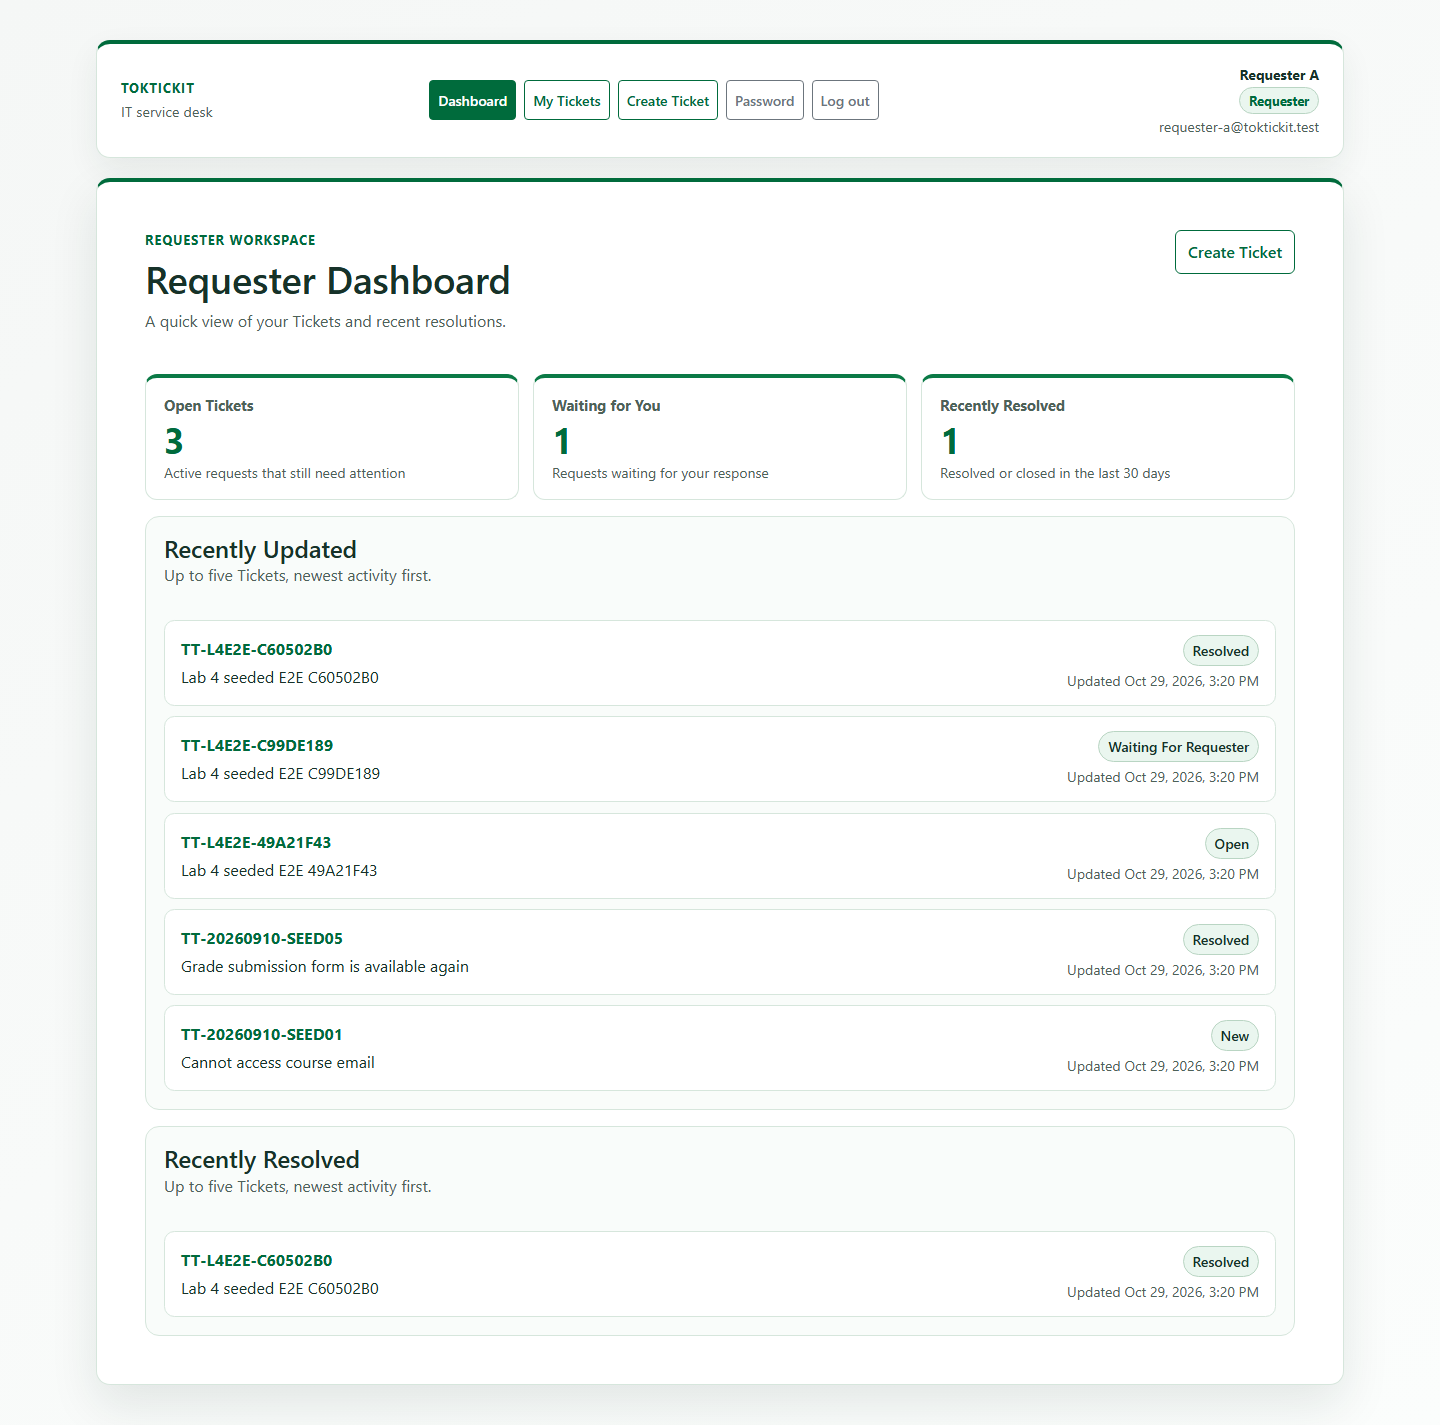
\includegraphics[width=\linewidth,height=0.40\textheight,keepaspectratio]{docs/lab-04/report/evidence/requester-dashboard-populated.png}
  \captionof{figure}{Seeded Requester dashboard with owned active, waiting, recently updated, and recently resolved Tickets.}
\end{minipage}\hfill
\begin{minipage}[t]{0.48\linewidth}\centering
  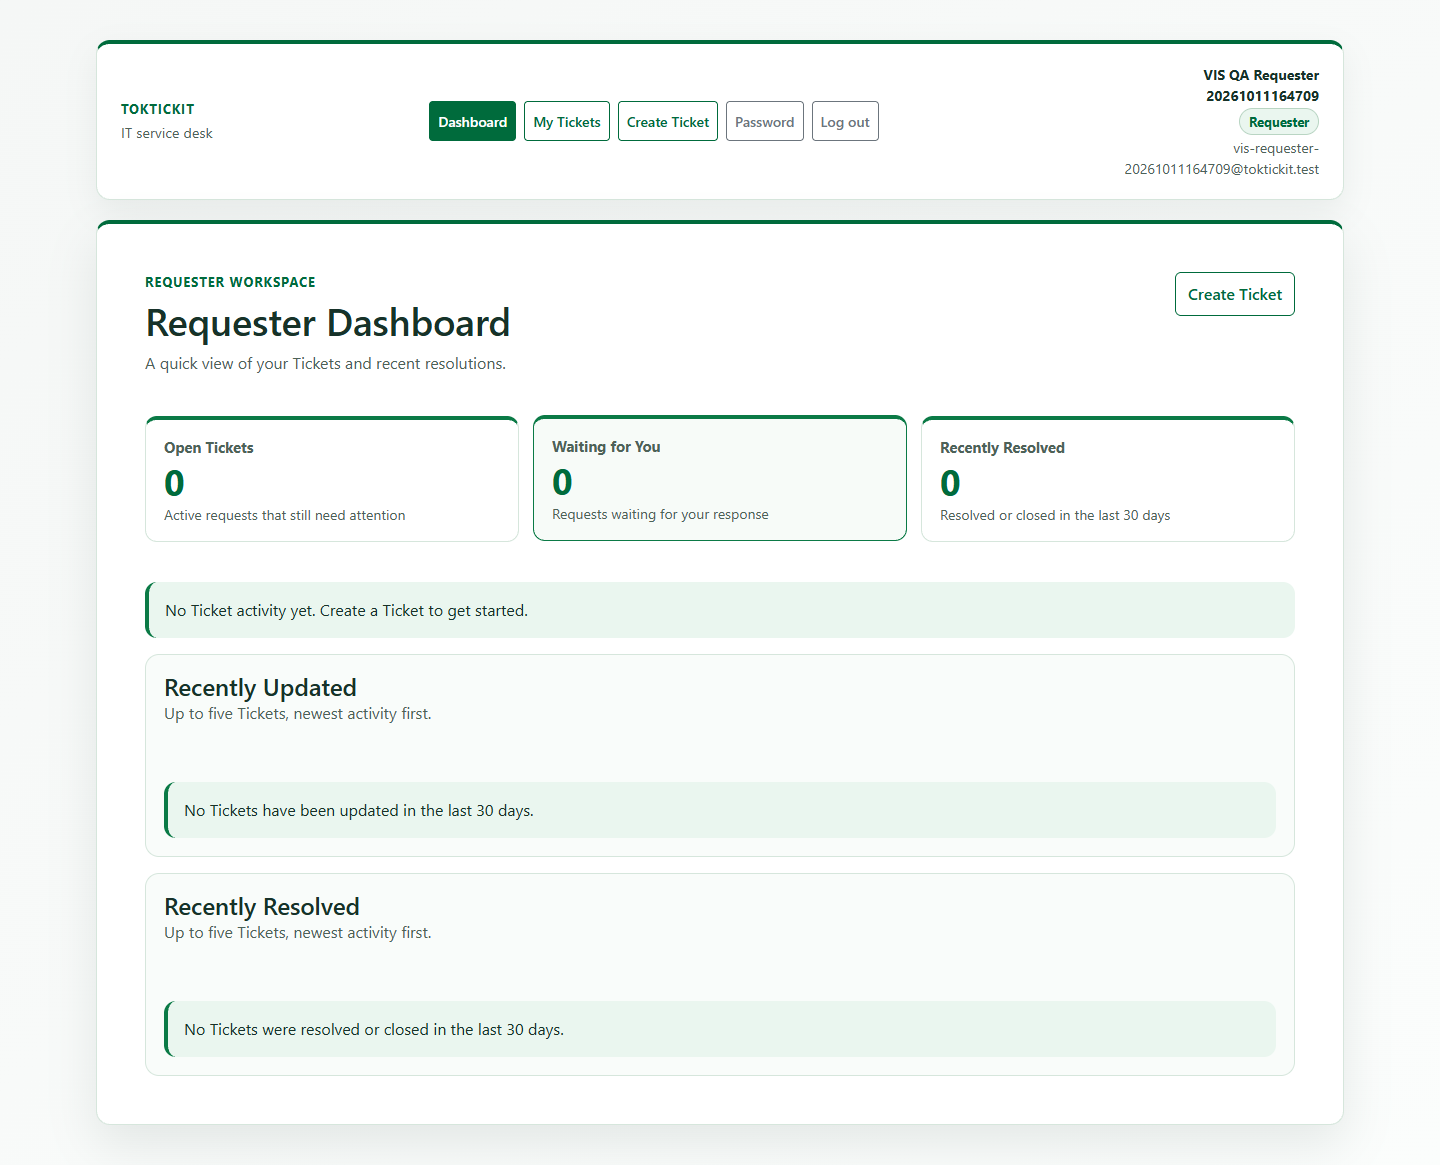
\includegraphics[width=\linewidth,height=0.40\textheight,keepaspectratio]{artifacts/lab-04/evidence/visual-inspection/requester-dashboard-1440x900.png}
  \captionof{figure}{Zero-data Requester dashboard with zero counts and explicit empty states.}
\end{minipage}

\smallskip
Counts and rows in the populated state are produced by the real API from isolated PostgreSQL fixtures; the empty state uses a Requester with no Tickets.

\answerpart{9}{Zen Green UI, Responsive, Accessibility, and Final Polish}

The UI preserves the Lab 3 Zen Green tokens and shared navigation. The rendered summary below and the linked full UI specification cover role navigation, dashboard cards, Actions Taken, loading/validation/empty/error feedback, and responsive behavior. VIS-01 records Requester, Staff, and Administrator routes at desktop (1440\,$\times$\,900), tablet (768\,$\times$\,1024), and mobile (390\,$\times$\,844), including dashboards, Ticket Detail, Staff Queue, Admin User Management, and Ticket Review. The owner-confirmed checklist records keyboard traversal, visible focus, semantic labels, announcements, non-color status cues, and no clipping, overlap, or horizontal overflow. Axe-core samples reported zero violations and zero incomplete checks on the sampled pages; screenshots alone do not establish authorization.

\begin{center}\small
\begin{tabularx}{\linewidth}{@{}p{43mm}YYY@{}}
\toprule
Screen & Desktop & Tablet & Mobile \\
\midrule
Requester Dashboard & \screenshotlink{artifacts/lab-04/evidence/visual-inspection/requester-dashboard-1440x900.png}{1440} & \screenshotlink{artifacts/lab-04/evidence/visual-inspection/requester-dashboard-768x1024.png}{768} & \screenshotlink{artifacts/lab-04/evidence/visual-inspection/requester-dashboard-390x844.png}{390} \\
IT Staff Dashboard & \screenshotlink{artifacts/lab-04/evidence/visual-inspection/it-staff-dashboard-1440x900.png}{1440} & \screenshotlink{artifacts/lab-04/evidence/visual-inspection/it-staff-dashboard-768x1024.png}{768} & \screenshotlink{artifacts/lab-04/evidence/visual-inspection/it-staff-dashboard-390x844.png}{390} \\
Requester Ticket Detail & \screenshotlink{artifacts/lab-04/evidence/visual-inspection/requester-ticket-detail-1440x900.png}{1440} & \screenshotlink{artifacts/lab-04/evidence/visual-inspection/requester-ticket-detail-768x1024.png}{768} & \screenshotlink{artifacts/lab-04/evidence/visual-inspection/requester-ticket-detail-390x844.png}{390} \\
IT Staff Ticket Detail & \screenshotlink{artifacts/lab-04/evidence/visual-inspection/it-staff-ticket-detail-1440x900.png}{1440} & \screenshotlink{artifacts/lab-04/evidence/visual-inspection/it-staff-ticket-detail-768x1024.png}{768} & \screenshotlink{artifacts/lab-04/evidence/visual-inspection/it-staff-ticket-detail-390x844.png}{390} \\
Staff Queue & \screenshotlink{artifacts/lab-04/evidence/visual-inspection/it-staff-ticket-queue-1440x900.png}{1440} & \screenshotlink{artifacts/lab-04/evidence/visual-inspection/it-staff-ticket-queue-768x1024.png}{768} & \screenshotlink{artifacts/lab-04/evidence/visual-inspection/it-staff-ticket-queue-390x844.png}{390} \\
Admin Dashboard & \screenshotlink{artifacts/lab-04/evidence/visual-inspection/administrator-dashboard-1440x900.png}{1440} & \screenshotlink{artifacts/lab-04/evidence/visual-inspection/administrator-dashboard-768x1024.png}{768} & \screenshotlink{artifacts/lab-04/evidence/visual-inspection/administrator-dashboard-390x844.png}{390} \\
Admin User Management & \screenshotlink{artifacts/lab-04/evidence/visual-inspection/administrator-user-management-1440x900.png}{1440} & \screenshotlink{artifacts/lab-04/evidence/visual-inspection/administrator-user-management-768x1024.png}{768} & \screenshotlink{artifacts/lab-04/evidence/visual-inspection/administrator-user-management-390x844.png}{390} \\
Admin Ticket Review & \screenshotlink{artifacts/lab-04/evidence/visual-inspection/administrator-ticket-review-1440x900.png}{1440} & \screenshotlink{artifacts/lab-04/evidence/visual-inspection/administrator-ticket-review-768x1024.png}{768} & \screenshotlink{artifacts/lab-04/evidence/visual-inspection/administrator-ticket-review-390x844.png}{390} \\
\bottomrule
\end{tabularx}
\end{center}

The table links to the full-frame source captures; the following grouped pages compare desktop, tablet, and mobile captures of the primary Lab 4 screens. Action Taken create/edit panels are captured at all three viewport sizes. Full-page images remain available through the VIS-01 links above. The full \reportlink{docs/lab-04/ui-spec.md}{UI specification}, \reportlink{docs/lab-04/evidence/visual-inspection-checklist.md}{completed visual/accessibility checklist}, \screenshotlink{artifacts/lab-04/e2e/e2e-04-hardening/run-report.json}{machine-readable E2E-04 report}, and full-resolution \href{https://github.com/ovenmakemeheat/toktickit/tree/bd8cecd63f1dd3386b0b7f2ffcf270805e0190f3/artifacts/lab-04/evidence/visual-inspection}{visual evidence directory} remain available in the repository.

\responsivescreens{Requester Dashboard}{docs/lab-04/report/evidence/viewport/requester-dashboard-desktop.png}{docs/lab-04/report/evidence/viewport/requester-dashboard-tablet.png}{docs/lab-04/report/evidence/viewport/requester-dashboard-mobile.png}
\responsivescreens{IT Staff Dashboard}{docs/lab-04/report/evidence/viewport/staff-dashboard-desktop.png}{docs/lab-04/report/evidence/viewport/staff-dashboard-tablet.png}{docs/lab-04/report/evidence/viewport/staff-dashboard-mobile.png}
\responsivescreens{Administrator Dashboard}{docs/lab-04/report/evidence/viewport/admin-dashboard-desktop.png}{docs/lab-04/report/evidence/viewport/admin-dashboard-tablet.png}{docs/lab-04/report/evidence/viewport/admin-dashboard-mobile.png}
\responsivescreens{Requester Ticket Detail}{docs/lab-04/report/evidence/viewport/requester-ticket-detail-desktop.png}{docs/lab-04/report/evidence/viewport/requester-ticket-detail-tablet.png}{docs/lab-04/report/evidence/viewport/requester-ticket-detail-mobile.png}
\responsivescreens{IT Staff Ticket Detail}{docs/lab-04/report/evidence/viewport/staff-ticket-detail-desktop.png}{docs/lab-04/report/evidence/viewport/staff-ticket-detail-tablet.png}{docs/lab-04/report/evidence/viewport/staff-ticket-detail-mobile.png}
\responsiveforms{Action Taken create form}{docs/lab-04/report/evidence/action-form-create-desktop.png}{docs/lab-04/report/evidence/action-form-create-tablet.png}{docs/lab-04/report/evidence/action-form-create-mobile.png}
\responsiveforms{Action Taken edit form}{docs/lab-04/report/evidence/action-form-edit-desktop.png}{docs/lab-04/report/evidence/action-form-edit-tablet.png}{docs/lab-04/report/evidence/action-form-edit-mobile.png}

\end{document}
